\section{Zużycie wody i poszczególnych czynników energetycznych}

Woda jest dostarczana wodociągami, a woda destylowana jest dostarczana przez firmę zewnętrzną.

Zapotrzebowane na wodę destylowaną do produkcji szamponów i odżywek wynosi 2594.395 i dziennie. Czyli ok. 26\,hl wody destylowanej dziennie. Woda z sieci wodociągowej jest zużywana na mycie urządzeń i powierzchni oraz potrzeby sanitarne.

\begin{figure}[h]
	\centering
	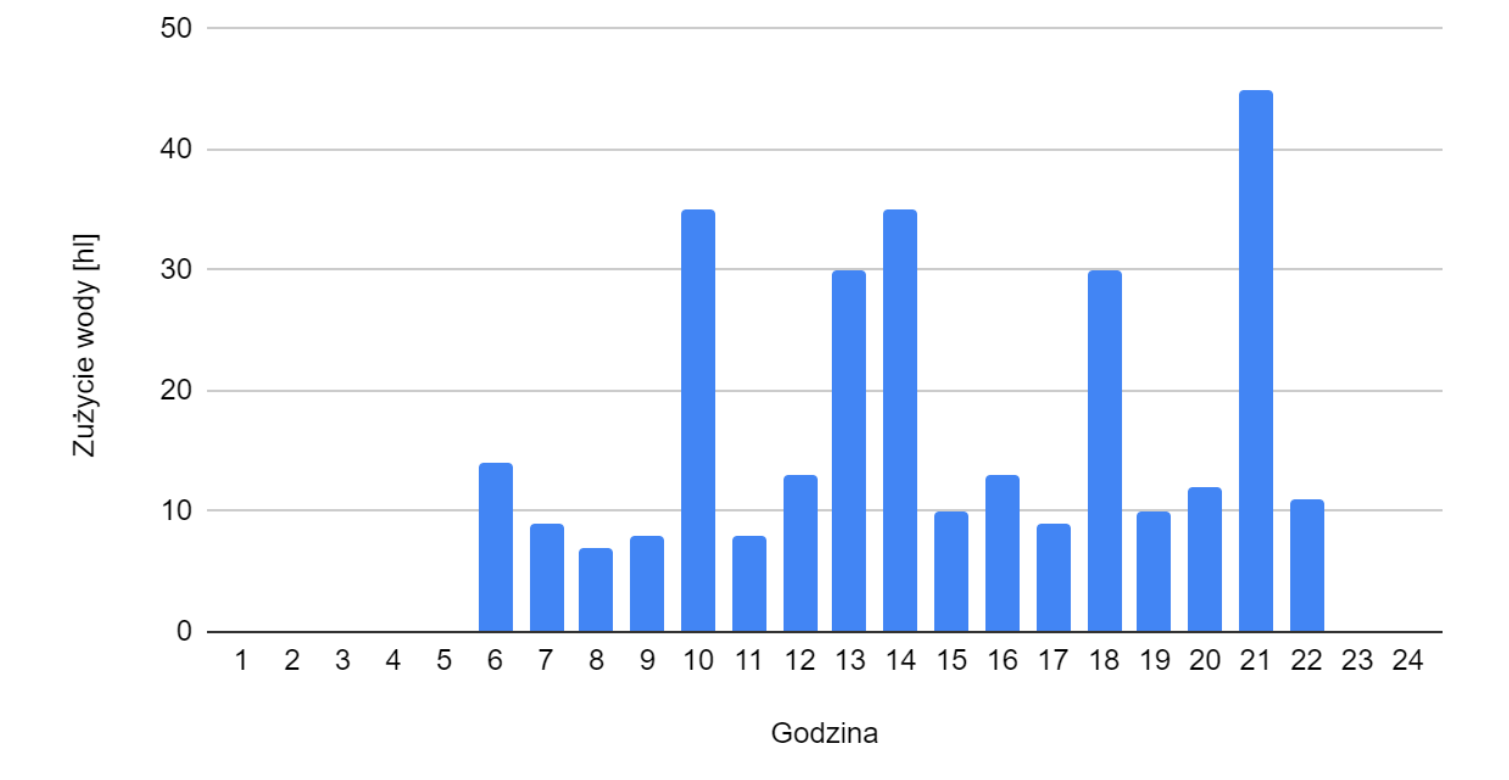
\includegraphics[width=0.8\textwidth]{./sec16/wykres1.png}
	\caption{Harmonogram zużycia wody w ciągu doby}
\end{figure}

Znacznie wyższe zużycie wody w danych godzinach jest spowodowane tym, że w tym czasie następuje mycie urządzeń oraz pompowanie wody potrzebnej do procesu technologicznego. Na koniec zmiany myte są urządzenia oraz podłogi i powierzchnie użytkowe. w dopieszczeniach. W godzinach zamknięcia zakładu woda nie jest zużywana. Są to wartości szacunkowe.

Zużycie energii elektrycznej w zakładzie nie jest zróżnicowane sezonowo. Wynika to z faktu, że latem energia zużywana podczas działania klimatyzacji jest porównywalna z energią zużywaną zimą na dogrzewanie pomieszczeń poprzez termowentylatory.  Zarówno latem i zimą energia jest zużywana podczas pracy maszyn ciągu technologicznego oraz oświetlenia zakładu. Średnie godzinowe zużycie energii wynosi 38.58\,kWh. W zakładzie średnio zużywa się 20$\mathrm{\frac{kW}{hl \text{ produkowanego szamponu lub odżywki}}}$.

\begin{figure}[h]
	\centering
	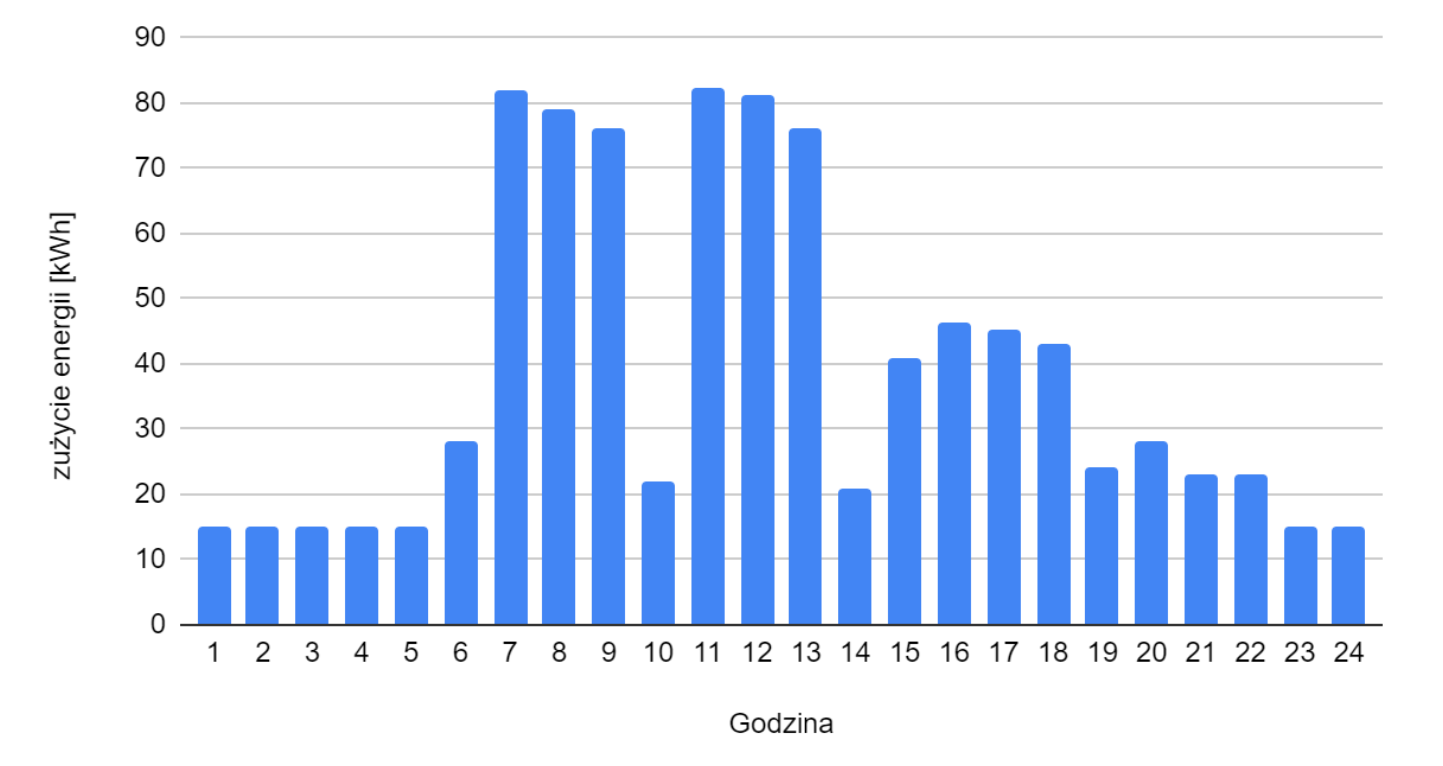
\includegraphics[width=0.8\textwidth]{./sec16/wykres2.png}
	\caption{Harmonogram zużycia energii elektrycznej dla poszczególnych godzin}
\end{figure}

Niskie zużycie energii w godzinach zamknięcia zakładu (22-6) wynika z braku pracy maszyn oraz minimalnego dogrzewania/klimatyzowania pomieszczeń przy jednoczesnym oświetleniu zewnętrznym budynku zakładu. Widoczny wzrost zużycia energii jest związany z pracą maszyn ciągu technologicznego.
